\documentclass[11pt]{article}
\usepackage[letterpaper,margin=0.92in]{geometry}
\usepackage[T1]{fontenc}
\usepackage{amsmath,amssymb,booktabs,tabularx,array,enumitem,float,tikz,natbib,graphicx,xcolor}
\usetikzlibrary{positioning,calc}
\usepackage[hidelinks]{hyperref}
\definecolor{inktwo}{HTML}{25324A}
\definecolor{private}{HTML}{3C8D5A}
\definecolor{consensus}{HTML}{B75D7A}
\definecolor{planner}{HTML}{3977A8}
\definecolor{market}{HTML}{C98B32}
\newcolumntype{Y}{>{\raggedright\arraybackslash}X}
\newcommand{\E}{\mathbb{E}}
\newcommand{\Prb}{\mathbb{P}}
\newcommand{\ArtifactNote}[1]{\par\vspace{2pt}{\scriptsize\color{inktwo!72}#1}}
\newcommand{\Evidence}[1]{\par\noindent\textbf{Evidence status.} #1\par}
\newcommand{\Boundary}[1]{\par\noindent\textbf{Boundary.} #1\par}
\sloppy
\title{\textbf{The Common-Source Trap}\\[0.35em]\large Endogenous Independent Evidence in Distributed Discovery}
\author{Yohei Nakajima\\Untapped Capital}
\date{July 2026}

\begin{document}
\maketitle

\begin{abstract}
When several searchers can use a free common signal or purchase independent
signals, the group may remain concentrated on the common source even though one
independent source raises net discovery. This paper studies that wedge in a
finite, exact source-choice model. For arbitrary finite team size $N\geq2$, it
derives each common-to-independent payoff threshold, proves that the thresholds
are strictly decreasing, and characterizes every weak pure source-count
equilibrium. The planner thresholds are also explicit. At the all-common
boundary, an equilibrium/planner wedge exists exactly for
$p(1-p)(N-1)/N\leq c<p(1-p)$, an interval of width $p(1-p)/N$. Exact
enumeration for $N=2,\ldots,8$ reproduces the formulas. The result is not a
universal under-acquisition theorem: at $N=3$, $p=4/5$, and $c=13/375$, the
unique equilibrium purchases two independent sources while the planner
purchases one. The paper uses that counterexample to separate source diversity,
action diversity, disclosure, and rewards. It relates the theorem to bounded
mechanism and architecture results and states experimental predictions without
claiming human evidence. Every numerical table and figure is generated from
checksum-validated immutable artifacts.
\end{abstract}

\noindent\textbf{Keywords:} information acquisition; strategic experimentation;
source diversity; collective search; public goods; distributed discovery.

\Evidence{The central threshold ordering and all-common interval are analytic
theorems (DD-C-0057). The $N=2,\ldots,8$ tables are exact finite
classifications (DD-C-0052). The interior over-acquisition fixture is an exact
negative result (DD-C-0058). DD-011 contributes synthetic predictions only; no
participant was recruited and no human experiment was conducted.}
\noindent\textbf{Publication status:} Working paper; not submitted, not peer
reviewed, and no DOI.

% Generated evidence asset; do not edit by hand.
% Claims: DD-C-0051, DD-C-0052, DD-C-0053, DD-C-0054, DD-C-0056, DD-C-0057, DD-C-0058
\begin{table}[t]\centering\small
\caption{Evidence layers used in this paper. Aggregation does not promote a claim's status.}
\label{tab:evidence-status}
\begin{tabularx}{\textwidth}{lXll}
\toprule Object & Result & Evidence category & Boundary\\\midrule
DD-008 & Two-agent trap interval & exact bounded grid & one frozen fixture family\\
DD-008A & $N=2,\ldots,8$ source counts & exact finite census & registered rational grid\\
DD-008B & decreasing thresholds and count characterization & analytic theorem & frozen homogeneous model\\
DD-008B & interior over-acquisition witness & exact negative result & one rational fixture\\
DD-006B & 16 strict mechanism rows & exhaustive exact class & subsidized, bounded transfers\\
DD-009 & 20 coherent architectures & bounded exact atlas & 288 declared cells only\\
DD-011 & design and power rows & synthetic estimate & no human experiment\\
\bottomrule\end{tabularx}
\ArtifactNote{Source runs: \path{20260721T141527Z_DD-008_0d11dc77_7e0c8f1d66, 20260721T163030Z_DD-008A_8b70668b_06307caab4, 20260721T192412Z_DD-008B_649deb08_29dbeaf3a9, 20260721T165512Z_DD-006B_f022a1a5_3be21d0b9b, 20260721T171249Z_DD-009_bc78d249_0c3851c41a, 20260721T185647Z_DD-011_fa0271d9_fcaa647c55}; claims: DD-C-0051, DD-C-0052, DD-C-0053, DD-C-0054, DD-C-0056, DD-C-0057, DD-C-0058; generator: \path{distributed_discovery.papers.build_common_source_trap}; input SHA-256 prefixes: \texttt{5e1da8ec2e34, 6df75b7bf2b1, a9d7c5143d75, a877471e9075, 34542e79cb88, acf90df6a2dc, 0d586f4001c8}.}
\end{table}


\section{Introduction}

Collective search often begins with a source decision. A research team chooses
which datasets, assays, experts, or models to consult before it chooses which
hypotheses to test. An investment team chooses whether to reuse a familiar
diligence channel or commission an independent view before it allocates capital.
A multi-agent system chooses whether several agents should retrieve the same
context or obtain conditionally independent evidence before they act. These
examples share a basic tension. A common source is cheap and makes individual
beliefs mutually predictable. An independent source is costly but can create a
new route to the target. The benefit of that new route is partly public, whereas
its cost is borne by the user who acquires it.

That tension has deep prior art. The distinction between private and social
value of information is classical \citep{Hirshleifer1971}. In strategic
experimentation, information produced by one player's risky action is a public
good, creating free-rider and encouragement effects
\citep{BoltonHarris1999,KellerRadyCripps2005}. Coordination motives can make
agents want to know what others know, while strategic substitution can instead
favor differentiated information \citep{HellwigVeldkamp2009}. Richer models
connect endogenous attention to source clarity, action complementarity, and
welfare \citep{MyattWallace2012,ColomboFemminisPavan2014}. Costly social
learning can strengthen herding \citep{Ali2018}; complementary correlated
sources can generate long-run learning traps \citep{LiangMu2020}. The broad
phenomenon of acquisition externalities is therefore not new.

The contribution here is narrower and exact. We isolate a one-shot finite model
in which $N$ agents select a free shared signal or a costly conditionally
independent signal, then search the signaled target directly. Correct searchers
split a unit prize. The planner values the union event that at least one searcher
is correct, minus acquisition costs. This creates a transparent mapping from
source choice to discovery coverage and permits exact type-payoff accounting.
The model removes social histories, dynamic experimentation, arbitrary signal
design, and strategic action choice. Those omissions make the theorem auditable;
they also define its limits.

The first result is a general finite-team threshold characterization. If $k$
agents currently use independent sources, a common user compares its shared
prize to the prize it would earn as the $(k+1)$st independent user. The gross
gain is
\[
 A_k=p(1-p)\E\left[\frac{1}{1+X_k}-\frac{1}{N-k+X_k}\right],
 \qquad X_k\sim\operatorname{Binomial}(k,p).
\]
The sequence $A_0,A_1,\ldots,A_{N-1}$ is strictly decreasing for every finite
$N\ge2$ and $0<p<1$. Consequently a count $k$ is a weak pure equilibrium if
and only if $A_k\le c\le A_{k-1}$, omitting the nonexistent boundary inequality.
The planner's corresponding gross thresholds are
$B_k=p(1-p)^{k+1}$ through $k=N-2$, followed by $B_{N-1}=0$.

At $k=0$, the comparison becomes especially clear:
\[
 A_0=p(1-p)\frac{N-1}{N}<p(1-p)=B_0.
\]
Thus all-common source use can remain an equilibrium when every planner optimum
uses at least one independent source. The exact interval has width
$p(1-p)/N$. This generalizes the two-agent Common-Source Trap while preserving
the earlier bounded $N=2,\ldots,8$ census as a separate computational result.

The second result limits the interpretation. The private and planner threshold
sequences are each decreasing, but they need not be globally ordered. For
$N=3$ and the transition from one to two independent sources,
$A_1=p(1-p)(3-2p)/6$ exceeds $B_1=p(1-p)^2$ exactly when $p>3/4$. At the
rational fixture $(p,c)=(4/5,13/375)$, private competition produces two
independent sources and the planner wants only one. This exact negative result
rules out a paper-wide claim that decentralized teams always under-acquire
independence.

The broader lesson is architectural. Source independence changes what evidence
exists. Disclosure changes who sees it. Allocation changes whether different
signals become different searches. Rewards change private incentives over both
reports and actions. A policy that repairs one margin can leave another margin
unchanged, and a source-diverse architecture can still collapse into a single
action after pooling. The paper therefore connects the source theorem to the
project's bounded mechanism, architecture, and experimental-design evidence
without treating those distinct models as one welfare theorem.

% Generated evidence asset; do not edit by hand.
% Claims: DD-C-0051, DD-C-0057
\begin{figure}[t]\centering
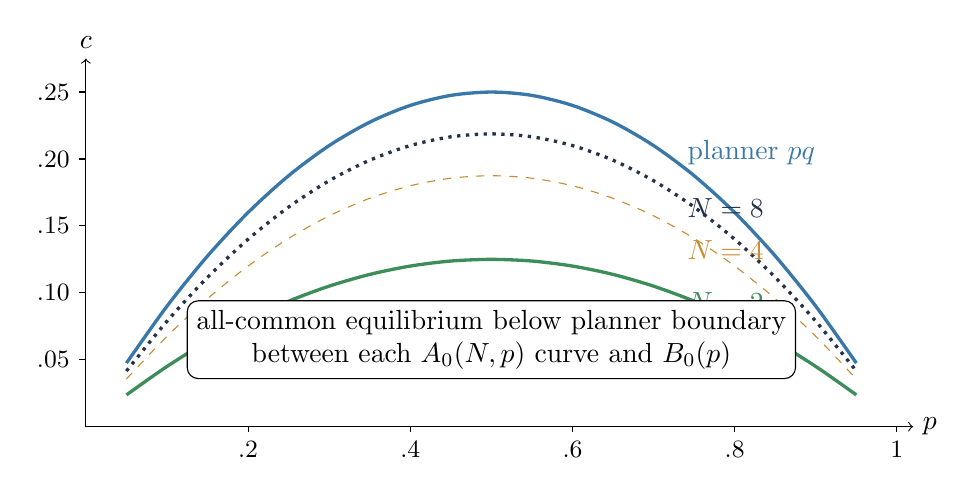
\begin{tikzpicture}[x=10.3cm,y=17cm]
\draw[->] (0,0)--(1.02,0) node[right] {$p$};
\draw[->] (0,0)--(0,.275) node[above] {$c$};
\foreach \x/\lab in {.2/{.2},.4/{.4},.6/{.6},.8/{.8},1/{1}} {\draw (\x,0)--(\x,-.004) node[below] {\small $\lab$};}
\foreach \y/\lab in {.05/{.05},.10/{.10},.15/{.15},.20/{.20},.25/{.25}} {\draw (0,\y)--(-.008,\y) node[left] {\small $\lab$};}
\draw[very thick,planner] plot[smooth] coordinates {(0.050,0.04750) (0.100,0.09000) (0.150,0.12750) (0.200,0.16000) (0.250,0.18750) (0.300,0.21000) (0.350,0.22750) (0.400,0.24000) (0.450,0.24750) (0.500,0.25000) (0.550,0.24750) (0.600,0.24000) (0.650,0.22750) (0.700,0.21000) (0.750,0.18750) (0.800,0.16000) (0.850,0.12750) (0.900,0.09000) (0.950,0.04750)};
\draw[very thick,private] plot[smooth] coordinates {(0.050,0.02375) (0.100,0.04500) (0.150,0.06375) (0.200,0.08000) (0.250,0.09375) (0.300,0.10500) (0.350,0.11375) (0.400,0.12000) (0.450,0.12375) (0.500,0.12500) (0.550,0.12375) (0.600,0.12000) (0.650,0.11375) (0.700,0.10500) (0.750,0.09375) (0.800,0.08000) (0.850,0.06375) (0.900,0.04500) (0.950,0.02375)};
\draw[dashed,market] plot[smooth] coordinates {(0.050,0.03563) (0.100,0.06750) (0.150,0.09563) (0.200,0.12000) (0.250,0.14062) (0.300,0.15750) (0.350,0.17062) (0.400,0.18000) (0.450,0.18562) (0.500,0.18750) (0.550,0.18562) (0.600,0.18000) (0.650,0.17062) (0.700,0.15750) (0.750,0.14062) (0.800,0.12000) (0.850,0.09563) (0.900,0.06750) (0.950,0.03563)};
\draw[dotted,inktwo,very thick] plot[smooth] coordinates {(0.050,0.04156) (0.100,0.07875) (0.150,0.11156) (0.200,0.14000) (0.250,0.16406) (0.300,0.18375) (0.350,0.19906) (0.400,0.21000) (0.450,0.21656) (0.500,0.21875) (0.550,0.21656) (0.600,0.21000) (0.650,0.19906) (0.700,0.18375) (0.750,0.16406) (0.800,0.14000) (0.850,0.11156) (0.900,0.07875) (0.950,0.04156)};
\node[planner,anchor=west] at (.73,.205) {planner $pq$};
\node[private,anchor=west] at (.73,.093) {$N=2$};
\node[market,anchor=west] at (.73,.132) {$N=4$};
\node[inktwo,anchor=west] at (.73,.163) {$N=8$};
\node[align=center,fill=white,draw,rounded corners] at (.50,.065) {all-common equilibrium below planner boundary\\between each $A_0(N,p)$ curve and $B_0(p)$};
\end{tikzpicture}
\caption{The exact all-common trap region. The upper curve is the planner's first-source threshold $B_0=p(1-p)$; lower curves are private thresholds $A_0=p(1-p)(N-1)/N$. The vertical width is $p(1-p)/N$.}
\label{fig:trap-region}
\ArtifactNote{Source runs: \path{20260721T141527Z_DD-008_0d11dc77_7e0c8f1d66, 20260721T192412Z_DD-008B_649deb08_29dbeaf3a9}; claims: DD-C-0051, DD-C-0057; generator: \path{distributed_discovery.papers.build_common_source_trap}; input SHA-256 prefixes: \texttt{5e1da8ec2e34, a9d7c5143d75}.}
\end{figure}


The remainder proceeds as follows. Section 2 positions the result against the
acquisition, learning, experimentation, and cognitive-labor literatures. Section
3 defines the model and accounting. Sections 4--8 present the two-agent result,
finite census, general theorem, planner comparison, and exact gap tables.
Sections 9--12 separate institutional remedies, joint mechanisms, architecture
choices, and experimental predictions. Section 13 records limitations, and
Section 14 concludes. Appendices collect proofs, finite-grid interpretation, and
reproducibility details.

\section{Related literature}

\subsection{Private and social value of information}

The starting point is the established distinction between the private return to
information and its social return. \citet{Hirshleifer1971} showed that private
information can redistribute rents rather than create commensurate social
value. Later information-acquisition work formalizes how strategic externalities
and the use of information create wedges between equilibrium and efficient
acquisition. \citet{ColomboFemminisPavan2014}, for example, separate
inefficiency in acquiring information from inefficiency in using it and show
that efficient use does not guarantee efficient acquisition. The current model
shares that separation but uses a different objective: one-shot union discovery
rather than a Gaussian-quadratic action economy.

Coordination motives also shape which sources agents choose.
\citet{HellwigVeldkamp2009} show that strategic complementarity can make
information choices complementary: agents may prefer to know what others know.
With strategic substitutes, differentiated information can instead become more
valuable. \citet{MyattWallace2012} study costly attention across signals that
differ in accuracy and clarity; stronger action complementarity can reduce the
number of attended signals and make acquired information more public. Those
models establish that common-source selection is endogenous to the payoff
technology. The exact thresholds below are a specialization to equal prize
splitting and direct coverage, not a substitute for those general frameworks.

\subsection{Strategic experimentation and information public goods}

In multi-agent bandit problems, current experimentation produces information
that others can use later. \citet{BoltonHarris1999} identify both a free-rider
effect and an encouragement effect: future experimentation by others can reduce
one's incentive to experiment, but it can also increase the value of bringing
information forward. \citet{KellerRadyCripps2005} find inefficiently low
experimentation rates under stationary Markov behavior and show that asymmetric
role patterns can improve efficiency. These are dynamic results with
continuation values, belief states, and endogenous timing. Our agents receive a
single signal and act once. The analogy is the public-good margin of independent
evidence, not the equilibrium object or welfare result.

The dynamic literature is nevertheless important for interpretation. A static
source subsidy can close a one-shot threshold gap while failing to solve a
dynamic experimentation problem. Conversely, role rotation can distribute the
burden of experimentation in a repeated setting even when a one-shot model
would assign a single independent source. The institutional section treats
assignment and rotation as distinct extensions precisely because the present
proof contains no repeated-game incentive.

\subsection{Costly herding, source choice, and learning traps}

Costly information creates a direct motive to free-ride on public histories.
\citet{Ali2018} characterizes when costly acquisition still permits complete
social learning; whether information can overturn the public history is central.
\citet{LiangMu2020} allow learners to choose among flexibly correlated sources
and characterize efficient aggregation versus long-run learning traps generated
by informational complementarities. Their agents arrive sequentially and pass
information across periods. The Common-Source Trap studied here has no public
history and no asymptotic learning criterion. It is a source-count equilibrium
inside a single coverage problem.

This distinction prevents a tempting but invalid inference. Common source use
in our model does not imply an incorrect herd. The shared signal is correct with
probability $p$, and the group may rationally accept concentration when
independence is expensive. Likewise, the phrase ``trap'' describes a precise
equilibrium/planner wedge, not an absorbing state in a social-learning process.
The value of the finite model is that the wedge, its width, and its disappearance
at a boundary are all explicit.

\subsection{Scientific and functional diversity}

The division of cognitive labor is a longstanding topic in philosophy and
science studies. \citet{Kitcher1990} analyzes how incentives can distribute
scientists across approaches. \citet{WeisbergMuldoon2009} use epistemic
landscapes to model exploration by heterogeneous scientific agents, and
\citet{Zollman2010} studies the value of transient diversity. Importantly,
\citet{AlexanderEtAl2015} challenge broad conclusions drawn from particular
landscape models and show that optimal search and the benefits of diversity are
sensitive to modeling choices. That disagreement supports the evidence policy
used here: define the target law, source structure, action map, and objective
before claiming that more diversity is better.

Functional diversity can also improve collective problem solving under specific
assumptions \citep{HongPage2004}, while coordinated experiment choice can reduce
redundant scientific search \citep{RzhetskyEtAl2015}. Those models involve
heuristics, topics, or experiment portfolios. Our source independence is much
narrower. Two agents can possess independent evidence yet take the same action;
agents can possess the same evidence yet be assigned different actions. Source
diversity and action diversity are therefore separate state variables.

Organizational architecture and parallel search provide additional direct
neighbors. Hierarchies and polyarchies alter screening errors
\citep{SahStiglitz1986}; communication networks can accelerate convergence while
reducing sustained exploration \citep{LazerFriedman2007}; and transparency can
change localized experimentation \citep{Bernstein2012}. Parallel R\&D and
uncoordinated-search models likewise make duplication a strategic or algorithmic
object \citep{BranderAmitAntweiler2002,KormanRodeh2020}. These works use
different error, timing, and payoff structures. The threshold proved here
belongs only to the frozen homogeneous equal-prize source-choice game.

\Boundary{The literature review supports adjacency statements, not a novelty
certificate. Information-acquisition externalities, public-good experimentation,
costly herding, source-choice coordination, and cognitive division of labor all
predate this paper. The new claim recorded here is only the exact theorem for the
declared coverage-and-prize model.}

\section{Model}

There are $N\ge2$ agents and three possible targets. The target
$\theta\in\{1,2,3\}$ is uniform. Before observing evidence, each agent chooses
one of two source types. The common source $C$ is free. Every agent selecting
$C$ observes the same draw. An independent source $I$ costs $c\ge0$ per user;
each $I$ user observes a distinct draw conditionally independent of every other
source given $\theta$. Every source has homogeneous accuracy $p\in(0,1)$:
\[
 \Prb(S=\theta\mid\theta)=p,
 \qquad
 \Prb(S=s\ne\theta\mid\theta)=\frac{1-p}{2}.
\]
Agents follow their clues directly, so action $a_i=S_i$. There is no report,
message, or contingent action policy. If at least one action equals the target,
a unit prize is split equally among correct agents. An incorrect agent receives
zero. The planner's gross discovery is the probability that the target appears
in the action union. Social net value subtracts the real acquisition cost $kc$
when $k$ agents use independent sources.

The source-count representation is lossless because agents of a given type are
symmetric. Let $k\in\{0,\ldots,N\}$ denote the number of $I$ users and
$m=N-k$ the number of $C$ users. For $k<N$, the group sees $k+1$ conditionally
independent source draws: $k$ individual draws plus one common draw. For $k=N$,
it sees $N$ draws. Hence gross discovery is
\begin{equation}
 G_N(k,p)=
 \begin{cases}
 1-(1-p)^{k+1}, & k<N,\\
 1-(1-p)^N, & k=N.
 \end{cases}
 \label{eq:discovery}
\end{equation}
The last independent purchase, from $k=N-1$ to $k=N$, creates no new source
draw; the sole remaining common user was already the sole user of that draw.

Let $X_r\sim\operatorname{Binomial}(r,p)$ count correct independent users among
$r$ other agents. A common user's gross payoff at a profile with $k<N$ is
\begin{equation}
 C_k=p\E\left[\frac{1}{N-k+X_k}\right].
 \label{eq:common-payoff}
\end{equation}
The common user receives a prize only if the common draw is correct; then all
$m=N-k$ common users are correct together and share with $X_k$ correct
independent users.

For $0<k<N$, an independent user's gross payoff is
\begin{equation}
 I_k=p\left[(1-p)\E\frac{1}{1+X_{k-1}}
 +p\E\frac{1}{N-k+1+X_{k-1}}\right].
 \label{eq:independent-payoff}
\end{equation}
When the common draw is wrong, the independent winner shares only with correct
independent peers. When it is correct, the $N-k$ common users join the prize.
At $k=N$, the second case collapses and
$I_N=p\E[1/(1+X_{N-1})]$. Net independent payoff is $I_k-c$.

Two accounting checks are useful. First,
\begin{equation}
 kI_k+(N-k)C_k=G_N(k,p),
 \label{eq:prize-accounting}
\end{equation}
with the absent type omitted. The prize paid across correct agents sums to one
exactly on the discovery event. Second, direct enumeration over the target and
all source-signal states reproduces equations
\eqref{eq:discovery}--\eqref{eq:prize-accounting}. The immutable DD-008A audit
performs that independent check on the registered finite grid (DD-C-0052).

\subsection{Equilibrium and planner conventions}

A source-count profile is a weak pure equilibrium if no $C$ user gains by
becoming an $I$ user and no $I$ user gains by becoming a $C$ user. It is strict
if both applicable inequalities are strict. Because individual identities do
not affect payoffs, a count classification covers every labeled profile at that
count. Ties are retained. At a threshold cost, adjacent source counts can both
be weak equilibria.

The planner chooses $k$ to maximize
\begin{equation}
 W_N(k,p,c)=G_N(k,p)-kc.
 \label{eq:welfare}
\end{equation}
Planner ties are also retained. The comparison does not add agents' prize
payments to social value; the unit prize is an internal transfer used to induce
private behavior. Discovery is the gross social objective and source costs are
real resource costs. Alternative accounting would define a different model.

\section{The two-agent Common-Source Trap}

With two agents there are three source counts. At $k=0$, common/common discovery
is $p$. A unilateral independent purchase creates a second conditionally
independent draw, so discovery becomes $2p-p^2$ and social net value becomes
$2p-p^2-c$. The planner therefore prefers one independent source exactly when
\begin{equation}
 c<p(1-p).
 \label{eq:two-planner}
\end{equation}

Private incentives are smaller at the all-common profile. Each common user
receives $p/2$. After deviating, the buyer is correct with probability $p$; it
receives the whole prize when the common draw is wrong and half when the common
draw is correct. Its gross payoff is
\[
 p(1-p)+\frac{p^2}{2}.
\]
The deviation gain before cost is $p(1-p)/2$. Thus common/common remains a weak
equilibrium exactly when
\begin{equation}
 c\ge\frac{p(1-p)}{2}.
 \label{eq:two-private}
\end{equation}
Combining \eqref{eq:two-planner} and \eqref{eq:two-private} yields the exact
two-agent trap interval
\begin{equation}
 \frac{p(1-p)}{2}\le c<p(1-p).
 \label{eq:two-trap}
\end{equation}

DD-008 evaluates a registered rational grid and checks the formulas by direct
target/signal enumeration. Five of its fifteen parameter cells fall in the
interval (DD-C-0051). That count is a property of the selected grid, while
equation \eqref{eq:two-trap} is the analytic boundary for the frozen two-agent
model. Neither statement estimates how real teams select evidence.

At the canonical illustrative accuracy $p=2/3$, the private threshold is $1/9$
and the planner threshold is $2/9$. The registered cost $c=1/8$ lies between
them. Common/common is then a strict source-choice equilibrium with discovery
$2/3$, whereas one independent source yields discovery $8/9$ and net value
$55/72>2/3$. The wedge is not caused by mistaken Bayesian updating: both source
laws and payoffs are common knowledge. It comes from prize sharing. The buyer
pays the full source cost but captures only part of the new union probability.

The name ``Common-Source Trap'' refers to this exact coexistence of a common-
source equilibrium and a planner preference for at least one independent
source. It does not mean that a common source is intrinsically bad. When cost is
high, all-common can be both equilibrium and planner optimal. When cost is low,
private users acquire independence. If robustness, common calibration, or
coordination has value outside the target-union objective, the planner boundary
would also change.

\section{Finite-team classification}

DD-008A extends the exact accounting to $N=2,\ldots,8$, accuracies
$p\in\{1/2,2/3,3/4\}$, and six rational costs. It evaluates 126
$(N,p,c)$ rows and every source count in each row. Closed-form binomial payoffs
are compared with a distinct direct enumerator over targets and source signals.
The two implementations agree in every cell, including prize conservation,
equilibrium status, and planner values (DD-C-0052).

The census preceded the general proof and remains useful for three reasons.
First, it is a regression suite for the payoff formulas. Second, it exposes ties
that a generic parameter argument can obscure. Third, it records how the
equilibrium and planner threshold crossings interact on a policy-relevant but
explicitly bounded rational grid. It is not the basis for the theorem's
unrestricted finite-$N$ quantifier.

\input{generated/equilibrium-counts.tex}

Figure \ref{fig:equilibrium-counts} reports the minimum weak-equilibrium count
at $p=2/3$. At zero cost, the minimum is $N-1$: once all but one users have
independent sources, the remaining common source is already an independent draw
and switching the last user is payoff-neutral. Positive costs reduce equilibrium
acquisition. At larger $N$, however, the count need not fall monotonically for a
fixed cost in a way that can be summarized by the all-common boundary alone;
interior prize competition matters.

% Generated evidence asset; do not edit by hand.
% Claims: DD-C-0052, DD-C-0057
\begin{figure}[t]\centering\small
\setlength{\tabcolsep}{7pt}
\begin{tabular}{ccccccc}
\toprule $N\backslash c$ & $0$ & $1/24$ & $1/12$ & $1/8$ & $1/6$ & $1/4$\\\midrule
2 & 2 & 1 & 1 & 1 & 1 & 0\\
3 & 3 & 2 & 1 & 1 & 1 & 0\\
4 & 4 & 2 & 1 & 1 & 1 & 0\\
5 & 5 & 2 & 1 & 1 & 1 & 0\\
6 & 6 & 2 & 1 & 1 & 1 & 0\\
7 & 7 & 2 & 1 & 1 & 1 & 0\\
8 & 8 & 2 & 1 & 1 & 1 & 0\\
\bottomrule\end{tabular}
\caption{Maximum planner-optimal independent-source count on the same registered grid.}
\label{fig:planner-counts}
\ArtifactNote{Source runs: \path{20260721T163030Z_DD-008A_8b70668b_06307caab4, 20260721T192412Z_DD-008B_649deb08_29dbeaf3a9}; claims: DD-C-0052, DD-C-0057; generator: \path{distributed_discovery.papers.build_common_source_trap}; input SHA-256 prefixes: \texttt{6df75b7bf2b1, a9d7c5143d75}.}
\end{figure}


The planner counts in Figure \ref{fig:planner-counts} follow the declining
marginal discovery increments. At zero cost, $N-1$ and $N$ tie, and the displayed
maximum is $N$. At any positive cost, $k=N$ is strictly dominated by $N-1$
because both have gross discovery $1-(1-p)^N$ but the former pays one additional
cost. This terminal redundancy is a consequence of defining a ``common source''
by its shared draw rather than by a fixed provider label.

The tables also show why a single statistic such as ``number of independent
sources'' is insufficient for welfare interpretation. A larger equilibrium
count may improve discovery but waste cost at the margin. A smaller count may
reflect an underprovided public good or an efficient response to expensive
signals. Exact threshold comparison is needed before assigning a sign.

\section{General finite-team thresholds}

We now state the general result established in DD-008B (DD-C-0057). Write
$q=1-p$. Consider a profile with $k<N$ independent users. A common user that
switches becomes an independent user in the $k+1$ profile. Let
\begin{equation}
 A_k=I_{k+1}-C_k
 \label{eq:ak-definition}
\end{equation}
denote the gross payoff gain before paying $c$. Substituting equations
\eqref{eq:common-payoff} and \eqref{eq:independent-payoff} and coupling the
other $k$ independent outcomes gives
\begin{equation}
 A_k=pq\E\left[\frac{1}{1+X_k}-\frac{1}{N-k+X_k}\right],
 \qquad X_k\sim\operatorname{Binomial}(k,p).
 \label{eq:ak}
\end{equation}

\paragraph{Theorem 1 (private thresholds and equilibrium counts).}
For every finite $N\ge2$ and $0<p<1$,
\[
 A_0>A_1>\cdots>A_{N-1}=0.
\]
A count $k\in\{0,\ldots,N\}$ is a weak pure source-count equilibrium if and
only if
\begin{equation}
 A_k\le c\le A_{k-1},
 \label{eq:equilibrium-characterization}
\end{equation}
where the left inequality is omitted at $k=N$ and the right inequality is
omitted at $k=0$.

The characterization follows directly from unilateral deviations. At count
$k$, a common user does not switch if $c\ge A_k$. An independent user does not
switch back if $c\le A_{k-1}$, because that reverse deviation compares the same
two adjacent source-count profiles. Strict threshold ordering then implies a
unique equilibrium count except at a threshold, where two adjacent counts are
weak equilibria.

The nontrivial step is monotonicity. Define
\[
 f_m(x)=\frac{1}{x+1}-\frac{1}{x+m},
 \qquad m=N-k.
\]
Couple $X_{k+1}=X_k+Y$ with $Y\sim\operatorname{Bernoulli}(p)$ independent.
Conditional on $X_k=x$,
\begin{align}
 f_m(x)-\E[f_{m-1}(x+Y)]
 =\frac{(x+1)(x+2)+p(m-2)(2x+m+1)}
 {(x+1)(x+2)(x+m-1)(x+m)}.
 \label{eq:positive-kernel}
\end{align}
For $m\ge2$, numerator and denominator are positive. Multiplying by $pq$ and
averaging proves $A_k>A_{k+1}$ for $k=0,\ldots,N-2$. Equation
\eqref{eq:ak} gives $A_{N-1}=0$.

The proof is analytic. The DD-008B executable audit instantiates 16,368
positive-kernel identities through $N=32$, matches 84 independently enumerated
private and planner margins through $N=5$, reproduces all 126 immutable DD-008A
classifications, and rejects altered threshold and census artifacts. Those
checks audit transcription and implementation; they do not replace the positive-
kernel proof.

\subsection{Boundary and large-team behavior}

At $k=0$, $X_0=0$, so equation \eqref{eq:ak} becomes
\begin{equation}
 A_0=pq\left(1-\frac1N\right).
 \label{eq:a0}
\end{equation}
For fixed $k$ and increasing $N$, the second reciprocal term in
\eqref{eq:ak} vanishes. Using
\[
 \E\frac{1}{1+X_k}=\frac{1-q^{k+1}}{(k+1)p}
\]
gives
\begin{equation}
 \lim_{N\to\infty}A_k=\frac{q(1-q^{k+1})}{k+1}.
 \label{eq:large-n}
\end{equation}
At fixed $k=0$, the private threshold approaches the planner's first-source
threshold from below. For interior fixed $k$, the limit need not lie below the
planner margin, foreshadowing the counterexample in Section 7.

\section{Planner comparison}

From equation \eqref{eq:discovery}, the planner's gross gain from the transition
$k\to k+1$ is
\begin{equation}
 B_k=G_N(k+1,p)-G_N(k,p)=
 \begin{cases}
 pq^{k+1}, & k=0,\ldots,N-2,\\
 0, & k=N-1.
 \end{cases}
 \label{eq:bk}
\end{equation}
The sequence is strictly decreasing through the positive margins. A planner
count $k$ is optimal if and only if $B_k\le c\le B_{k-1}$, with the same
boundary conventions. Thus equilibrium and planner counts are generated by two
ordered threshold sequences. The source-choice problem is not computationally
hard once those sequences are known; the economic content lies in their
differences.

\paragraph{Corollary 1 (general all-common trap).}
For every finite $N\ge2$ and $0<p<1$, all-common source use is a weak
equilibrium while every planner optimum uses at least one independent source
exactly when
\begin{equation}
 pq\frac{N-1}{N}\le c<pq.
 \label{eq:general-trap}
\end{equation}
The interval has width $pq/N$.

The lower endpoint is included because at $c=A_0$ the all-common profile is a
weak equilibrium. The upper endpoint is excluded because at $c=B_0$ the planner
is indifferent between zero and one independent source; not every planner
optimum then uses independence. If one instead asked whether at least one
planner optimum uses independence, the endpoint convention would differ. The
paper uses the stronger ``every planner optimum'' statement.

The width shrinks with $N$, but this does not mean that all private/planner
differences vanish in large teams. It only describes the first transition away
from the all-common boundary. As $N$ increases at fixed $p$, $A_0$ rises toward
$B_0$. A fixed cost strictly below $pq$ therefore eventually falls below the
private threshold, making all-common unstable. Interior thresholds can behave
differently because prize competition among already independent users changes
the private value of an additional source.

\subsection{An exact counterexample to universal under-acquisition}

For $N=3$ and $k=1$, equation \eqref{eq:ak} simplifies to
\begin{equation}
 A_1=\frac{pq(3-2p)}{6},
 \qquad B_1=pq^2.
 \label{eq:n3-interior}
\end{equation}
Their difference changes sign at $p=3/4$: $A_1>B_1$ exactly when $p>3/4$.
Set $p=4/5$ and $c=13/375$. Then
\[
 A_1=\frac{14}{375}>\frac{13}{375}>
 \frac{12}{375}=B_1.
\]
Since the threshold sequences are decreasing, the unique equilibrium count is
$k=2$ and the unique planner count is $k=1$ (DD-C-0058). Direct target/signal
enumeration reproduces both payoffs and rejects a corrupted threshold.

The mechanism is rent competition rather than a discovery externality with a
fixed sign. Moving from one to two independent users changes how a prospective
buyer shares the prize with common and independent winners. When accuracy is
high, avoiding the block of common winners can raise private prize share even
after the planner's incremental union probability has become small. The exact
example does not show that over-acquisition is typical. It shows that the phrase
``the Common-Source Trap'' cannot stand for a universal equilibrium ordering at
every interior count.

\section{Acquisition, discovery, and welfare gaps}

The DD-008A census records three related but distinct differences. The
\emph{independence gap} compares source counts. The \emph{discovery gap}
compares union probabilities. The \emph{welfare gap} compares net planner value
with net value at a selected equilibrium count. Conflating these gaps can reverse
an interpretation. More independent sources may increase discovery while
reducing net value; equal source counts can still support different action
technologies in a richer architecture.

% Generated evidence asset; do not edit by hand.
% Claims: DD-C-0052, DD-C-0057
\begin{figure}[t]\centering\small
\setlength{\tabcolsep}{7pt}
\begin{tabular}{ccccccc}
\toprule $N\backslash c$ & $0$ & $1/24$ & $1/12$ & $1/8$ & $1/6$ & $1/4$\\\midrule
2 & 1 & 0 & 0 & 1 & 1 & 0\\
3 & 1 & 0 & 0 & 0 & 1 & 0\\
4 & 1 & 0 & -1 & 0 & 1 & 0\\
5 & 1 & -1 & -1 & 0 & 0 & 0\\
6 & 1 & -1 & -1 & 0 & 0 & 0\\
7 & 1 & -2 & -1 & 0 & 0 & 0\\
8 & 1 & -2 & -1 & 0 & 0 & 0\\
\bottomrule\end{tabular}
\caption{Registered independence gap: maximum planner count minus minimum weak-equilibrium count.}
\label{fig:independence-gap}
\ArtifactNote{Source runs: \path{20260721T163030Z_DD-008A_8b70668b_06307caab4, 20260721T192412Z_DD-008B_649deb08_29dbeaf3a9}; claims: DD-C-0052, DD-C-0057; generator: \path{distributed_discovery.papers.build_common_source_trap}; input SHA-256 prefixes: \texttt{6df75b7bf2b1, a9d7c5143d75}.}
\end{figure}


Figure \ref{fig:independence-gap} uses the DD-008A convention: maximum planner
count minus minimum weak-equilibrium count. Positive values highlight a possible
under-acquisition comparison. Negative entries are not errors; they preserve
interior over-acquisition on the registered grid. At ties, the max/min convention
deliberately displays the widest count wedge and should not be confused with an
equilibrium-selection prediction.

% Generated evidence asset; do not edit by hand.
% Claims: DD-C-0052, DD-C-0057
\begin{figure}[t]\centering\scriptsize
\setlength{\tabcolsep}{5pt}
\begin{tabular}{ccccccc}
\toprule $N\backslash c$ & $0$ & $1/24$ & $1/12$ & $1/8$ & $1/6$ & $1/4$\\\midrule
2 & $0$ & $0$ & $0$ & $2/9$ & $2/9$ & $0$\\
3 & $0$ & $0$ & $0$ & $0$ & $2/9$ & $0$\\
4 & $0$ & $0$ & $-2/27$ & $0$ & $2/9$ & $0$\\
5 & $0$ & $-2/81$ & $-2/27$ & $0$ & $0$ & $0$\\
6 & $0$ & $-2/81$ & $-2/27$ & $0$ & $0$ & $0$\\
7 & $0$ & $-8/243$ & $-2/27$ & $0$ & $0$ & $0$\\
8 & $0$ & $-8/243$ & $-2/27$ & $0$ & $0$ & $0$\\
\bottomrule\end{tabular}
\caption{Gross discovery at the maximum planner count minus gross discovery at the minimum weak-equilibrium count. Negative cells are retained.}
\label{fig:discovery-gap}
\ArtifactNote{Source runs: \path{20260721T163030Z_DD-008A_8b70668b_06307caab4, 20260721T192412Z_DD-008B_649deb08_29dbeaf3a9}; claims: DD-C-0052, DD-C-0057; generator: \path{distributed_discovery.papers.build_common_source_trap}; input SHA-256 prefixes: \texttt{6df75b7bf2b1, a9d7c5143d75}.}
\end{figure}


Discovery is a monotone function of $k$ through $N-1$, but the last transition
is redundant. Figure \ref{fig:discovery-gap} therefore translates count gaps
into the target-union objective. A negative entry means the displayed minimum
equilibrium count yields greater gross discovery than the displayed maximum
planner count; this can occur only because the planner is accounting for cost.
It is not a claim that the planner prefers less discovery as an intrinsic good.

% Generated evidence asset; do not edit by hand.
% Claims: DD-C-0052, DD-C-0057
\begin{figure}[t]\centering\scriptsize
\setlength{\tabcolsep}{5pt}
\begin{tabular}{ccccccc}
\toprule $N\backslash c$ & $0$ & $1/24$ & $1/12$ & $1/8$ & $1/6$ & $1/4$\\\midrule
2 & $0$ & $0$ & $0$ & $7/72$ & $1/18$ & $0$\\
3 & $0$ & $0$ & $0$ & $0$ & $1/18$ & $0$\\
4 & $0$ & $0$ & $1/108$ & $0$ & $1/18$ & $0$\\
5 & $0$ & $11/648$ & $1/108$ & $0$ & $0$ & $0$\\
6 & $0$ & $11/648$ & $1/108$ & $0$ & $0$ & $0$\\
7 & $0$ & $49/972$ & $1/108$ & $0$ & $0$ & $0$\\
8 & $0$ & $49/972$ & $1/108$ & $0$ & $0$ & $0$\\
\bottomrule\end{tabular}
\caption{Planner net value minus net value at the minimum weak-equilibrium count. The planner definition makes every entry weakly nonnegative.}
\label{fig:welfare-gap}
\ArtifactNote{Source runs: \path{20260721T163030Z_DD-008A_8b70668b_06307caab4, 20260721T192412Z_DD-008B_649deb08_29dbeaf3a9}; claims: DD-C-0052, DD-C-0057; generator: \path{distributed_discovery.papers.build_common_source_trap}; input SHA-256 prefixes: \texttt{6df75b7bf2b1, a9d7c5143d75}.}
\end{figure}


The welfare gaps in Figure \ref{fig:welfare-gap} are weakly nonnegative by
construction because the planner count maximizes equation \eqref{eq:welfare}.
They can be zero even when source counts differ, either because of a tie or
because cost and discovery changes exactly offset. This table is the proper
place to discuss inefficiency on the registered grid. The count and discovery
tables diagnose mechanisms; the welfare table records the objective actually
optimized by the planner.

Three reporting choices matter. First, exact fractions are retained rather than
rounded decimals. Second, all registered costs remain visible, including null,
tied, and negative-gap cells. Third, the grid is not interpolated into an
empirical response surface. The general theorem supplies analytic threshold
boundaries, while the finite tables serve as auditable examples and regressions.

\section{Institutional remedies}

An acquisition wedge suggests several possible interventions, but they act on
different primitives. A source subsidy lowers the private cost of independence.
An assignment rule replaces source choice with an organizational decision. A
rotation rule distributes acquisition burden over time. Attribution or priority
protection changes the private return to producing evidence. Disclosure changes
who observes acquired evidence. Allocation changes how evidence becomes search
actions. A joint reward can make truth-telling and differentiated action
privately attractive. These instruments should not be treated as aliases.

At the all-common boundary, a per-independent-source subsidy $s$ changes the
private condition to $c-s<A_0$. The smallest strict subsidy is any
$s>c-A_0$ when $c\ge A_0$. If the planner wants the first independent source,
$c<B_0$, then the set of subsidies that strictly induce a unilateral purchase is
nonempty. This is a local implementation observation, not a budget-balance
result. Subsidy finance and selection among multiple buyers are outside the
model.

Assignment is mechanically stronger. A planner can designate exactly $k^star$
independent users and thereby attain the source-count optimum without changing
private source rewards. Yet assignment creates participation and observability
questions. Can the organization verify that the source is independent? Can it
observe source cost? Is an assigned user compensated? Does the source remain
independent after preprocessing or shared prompts? Those questions are absent
from the theorem and must be specified in an implementation model.

Priority and attribution can change the private return to evidence production.
The science literature emphasizes that incentives help allocate cognitive labor
across approaches \citep{Kitcher1990}. Experimental work also shows that
competition for novelty can change sampling behavior \citep{TiokhinDerex2019}.
But the sign is not automatic. Strong priority rewards can induce duplicated
races, premature disclosure avoidance, or the exact kind of interior
over-acquisition identified above. An intervention should therefore target a
declared estimand rather than ``more diversity'' in the abstract.

% Generated evidence asset; do not edit by hand.
% Claims: DD-C-0051, DD-C-0053, DD-C-0057
\begin{figure}[t]\centering
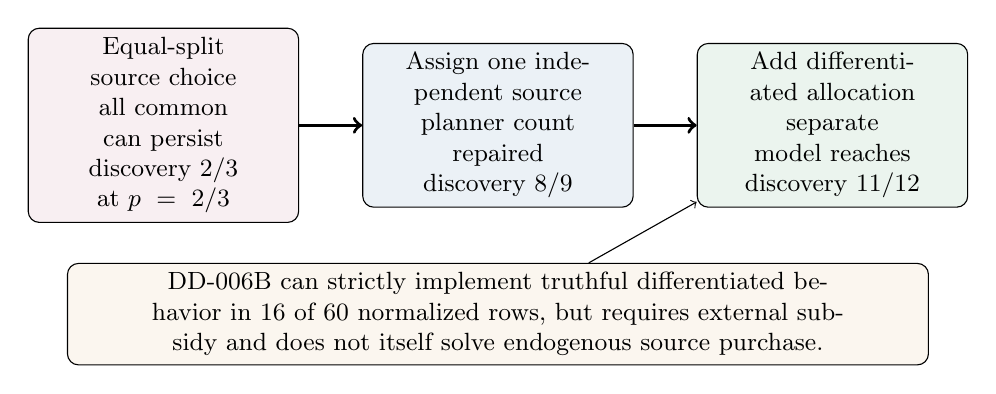
\begin{tikzpicture}[node distance=7mm and 8mm,every node/.style={align=center,font=\small}]
\node[draw,rounded corners,fill=consensus!10,text width=3.2cm] (base) {Equal-split source choice\\all common can persist\\discovery $2/3$ at $p=2/3$};
\node[draw,rounded corners,fill=planner!10,text width=3.2cm,right=of base] (assign) {Assign one independent source\\planner count repaired\\discovery $8/9$};
\node[draw,rounded corners,fill=private!10,text width=3.2cm,right=of assign] (alloc) {Add differentiated allocation\\separate model reaches\\discovery $11/12$};
\draw[->,very thick] (base)--(assign);
\draw[->,very thick] (assign)--(alloc);
\node[draw,rounded corners,fill=market!8,text width=10.7cm,below=of assign] (reward) {DD-006B can strictly implement truthful differentiated behavior in 16 of 60 normalized rows, but requires external subsidy and does not itself solve endogenous source purchase.};
\draw[->] (reward)--(alloc);
\end{tikzpicture}
\caption{Interventions repair different margins. DD-006B's maximum exact strict margin is $13/72$ and best strict discovery is $11/12$; those results use a different two-agent observability/transfer model.}
\label{fig:interventions}
\ArtifactNote{Source runs: \path{20260721T141527Z_DD-008_0d11dc77_7e0c8f1d66, 20260721T165512Z_DD-006B_f022a1a5_3be21d0b9b, 20260721T192412Z_DD-008B_649deb08_29dbeaf3a9}; claims: DD-C-0051, DD-C-0053, DD-C-0057; generator: \path{distributed_discovery.papers.build_common_source_trap}; input SHA-256 prefixes: \texttt{5e1da8ec2e34, 34542e79cb88, a877471e9075}.}
\end{figure}


Figure \ref{fig:interventions} emphasizes sequencing. Acquisition repair creates
distinct evidence. Allocation repair turns evidence into distinct actions. A
joint mechanism may additionally support truthful reports and obedience. The
numbers come from different registered models and are not additive. In
particular, $8/9$ in the acquisition fixture and $11/12$ in the differentiated
allocation fixture do not describe successive outcomes of one unified game.

\section{Joint truth and allocation mechanisms}

Source acquisition is only the first layer of distributed discovery. Once
evidence exists, agents may report strategically or ignore recommended actions.
DD-006B studies a separate two-agent, three-target mechanism class with
conditionally independent $2/3$-accurate signals, a normalized grid of score,
obedience, and coverage components, and four observability regimes. It exhausts
60 mechanism rows and 57,600 unilateral report/action deviations.

Sixteen rows strictly implement truthful reporting and a differentiated
recommendation for both fixed tie roles. The maximum exact all-tie margin is
$13/72$, and truthful differentiated discovery is $11/12$ (DD-C-0053). No weak
row exists when the target is hidden and actions are observed only through the
restricted target-hidden/action-hidden regime. These are exact results for the
registered normalized class, not a dominant-strategy theorem or an arbitrary-
transfer characterization.

The mechanism is also externally subsidized. Minimum strict expected subsidy in
the best regime is positive, and the Architecture Atlas accounts for transfer
budgets separately from discovery. Consequently DD-006B cannot be cited as a
free cure for the source-choice wedge. It begins after independent evidence is
already present and studies incentives to report and act. A complete mechanism
would need to combine acquisition, reporting, action, source verification, and
budget balance in one game.

This separation creates a useful research agenda. A source subsidy can induce
independence but may leave reports untruthful. A truthful scoring component can
elicit reports but leave both agents taking the same action. A marginal-coverage
component can reward differentiated action but may require target or action
observability unavailable in practice. Each result should travel with its
information requirements.

The DD-006B result is therefore best read as a feasibility witness. It proves
that strict joint truth/allocation incentives are possible in a bounded
subsidized class under sufficiently rich observability. It does not prove that a
specific organization can implement them, that the mechanism is budget-balanced,
or that people will comply. The experimental design in Section 12 treats
compliance as an open prediction.

\section{Architecture Atlas implications}

DD-009 places acquisition inside a bounded Cartesian architecture space. Its
declared dimensions are evidence, disclosure, allocation, timing, and reward.
Validity rules classify all 288 combinations; 20 coherent cells are evaluated
exactly and 268 are rejected with machine-readable reasons. Twelve evaluated
cells are nondominated under six fixed objectives. This is a bounded Atlas, not
a universal ranking (DD-C-0054).

% Generated evidence asset; do not edit by hand.
% Claims: DD-C-0054
\begin{figure}[t]\centering\scriptsize
\begin{tabularx}{\textwidth}{lXXXXX}
\toprule ID & Disclosure/allocation & Reward & Discovery & Net value & Boundary\\\midrule
A145 & private/direct & equal-split & $8/9$ & $23/36$ & protocol/selection\\
A199 & private/sequential & equal-split & $11/12$ & $2/3$ & protocol/selection\\
A209 & private/joint & DD-006A & $11/12$ & $2/3$ & weak mechanism\\
A210 & private/joint & DD-006B & $11/12$ & $-13/12$ & strict subsidized\\
A229 & pooled/consensus & equal-split & $2/3$ & $5/12$ & protocol/selection\\
A254 & pooled/planner & pooling & $11/12$ & $2/3$ & protocol/selection\\
\bottomrule\end{tabularx}
\caption{Acquisition-related slice of the bounded DD-009 Architecture Atlas. Every row uses two independent channels and cost $1/4$; changing disclosure, allocation, timing, and rewards changes discovery, net value, and incentive status. This is not a universal architecture ranking.}
\label{fig:atlas-slice}
\ArtifactNote{Source runs: \path{20260721T171249Z_DD-009_bc78d249_0c3851c41a}; claims: DD-C-0054; generator: \path{distributed_discovery.papers.build_common_source_trap}; input SHA-256 prefixes: \texttt{acf90df6a2dc}.}
\end{figure}


The acquisition slice in Figure \ref{fig:atlas-slice} holds two independent
channels and information cost $1/4$ fixed. Direct private action yields discovery
$8/9$. Sequential action or planner-style differentiated allocation yields
$11/12$. Pooling followed by consensus collapses discovery back to $2/3$
despite the independent sources. This is the source/action distinction in its
clearest form: acquiring independent evidence is not sufficient if the action
protocol compresses it.

Reward changes can also alter accounting without changing discovery. A sole-
rescue or marginal-coverage transfer can use budget while preserving the same
direct actions. The DD-006A row weakly supports truth and obedience with zero
recorded transfer budget under its restricted accounting; the DD-006B row is
strict but carries a large external budget. Those rows are not ordered by one
score. The Atlas retains discovery, social net value, transfer budget,
truthfulness, obedience, action quality, and operating quantities separately.

The Atlas also prevents favorable cherry-picking. A claim that ``independent
evidence plus pooling works'' must specify the allocation rule. A claim that a
joint mechanism is preferable must include its subsidy and observability. A
claim that sequential action improves discovery must report expected rounds and
actions. The relevant architecture is a tuple, not a label.

For the Common-Source theorem, the implication is modest. Acquisition thresholds
determine how many independent sources arise under one private reward. They do
not determine how those sources are disclosed or allocated. The theorem can be
used as an acquisition module inside a richer architecture only after the richer
model proves that downstream behavior does not feed back into source payoffs.

\section{Experimental predictions}

DD-011 translates the project's exact mechanisms into a preregistration-ready
synthetic design. The selected design has 20 treatment cells spanning acquisition,
attribution, disclosure, action timing, and rewards. It registers eight
hypotheses, fifteen outcomes, eight explicit synthetic response scenarios, and
six sample sizes. A seeded 384,000-draw Monte Carlo run reports conditional power
and minimum detectable effects; a separate verifier recreates every random
stream (DD-C-0056).

% Generated evidence asset; do not edit by hand.
% Claim: DD-C-0056
\begin{figure}[t]\centering
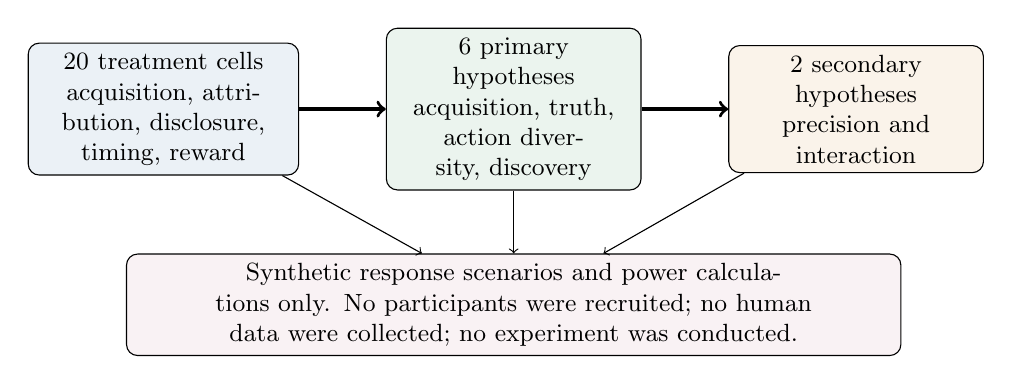
\begin{tikzpicture}[node distance=8mm and 11mm,every node/.style={align=center,font=\small}]
\node[draw,rounded corners,fill=planner!10,text width=3.2cm] (factors) {20 treatment cells\\acquisition, attribution, disclosure, timing, reward};
\node[draw,rounded corners,fill=private!10,text width=3.0cm,right=of factors] (primary) {6 primary hypotheses\\acquisition, truth, action diversity, discovery};
\node[draw,rounded corners,fill=market!10,text width=3.0cm,right=of primary] (secondary) {2 secondary hypotheses\\precision and interaction};
\draw[->,very thick] (factors)--(primary);
\draw[->,very thick] (primary)--(secondary);
\node[draw,rounded corners,fill=consensus!8,text width=9.6cm,below=of primary] (warning) {Synthetic response scenarios and power calculations only. No participants were recruited; no human data were collected; no experiment was conducted.};
\draw[->] (factors)--(warning); \draw[->] (primary)--(warning); \draw[->] (secondary)--(warning);
\end{tikzpicture}
\caption{DD-011 maps exact-model mechanisms into experimental predictions without turning them into empirical effects. The design is preregistration-ready, not preregistered or deployed.}
\label{fig:experiment-map}
\ArtifactNote{Source runs: \path{20260721T185647Z_DD-011_fa0271d9_fcaa647c55}; claims: DD-C-0056; generator: \path{distributed_discovery.papers.build_common_source_trap}; input SHA-256 prefixes: \texttt{0d586f4001c8}.}
\end{figure}


The source-choice predictions are straightforward to state but remain untested.
First, costly independent evidence may be under-acquired relative to assignment
in parameter cells near the all-common boundary. Second, assignment should
mechanically raise the rate of independent-source use, but its effect on
discovery depends on downstream action allocation. Third, source provenance may
help participants interpret reports, yet it need not increase truthful reporting
without attribution or verification. Fourth, acquisition and marginal-coverage
allocation may be complementary because the former creates diverse evidence and
the latter rewards diverse actions.

The exact model does not supply behavioral effect sizes. DD-011 therefore uses
declared synthetic assumptions rather than treating theorem differences as human
treatment effects. Under its rational synthetic scenario, all eight assumed
effects reach estimated power at least $0.80$ by total sample size 960, while 140
of 192 rows at sample sizes 640 or greater remain retained calibration failures
across all scenarios. Those failures are evidence about sensitivity of the
simulation design, not evidence that a real experiment is infeasible.

Several observations would be especially informative. If participants acquire
more independence than the planner benchmark in high-accuracy interior cells,
that would echo DD-C-0058 rather than falsify the entire framework. If public
disclosure raises agreement but not discovery, that would support separating
information and allocation. If a joint mechanism improves reports but not
obedience, it would locate the failure at the action layer. If provenance changes
confidence but not source choice, it would separate interpretability from
acquisition incentives.

\Boundary{No participants were recruited. No human data were collected. No
experiment was conducted. Separate ethics and institutional review are required
before deployment. The materials are an unsubmitted preregistration-ready kit,
not a preregistration or a claim of empirical power.}

\section{Limitations}

The first limitation is external validity. Every result in the core model is
mathematical evidence about a synthetic finite game. No dataset establishes that
research teams, firms, investors, or multi-agent systems face homogeneous
three-target signals, equal prize splitting, or direct clue-following. The model
is diagnostic: it shows that a source-choice wedge can arise under transparent
conditions and identifies the precise margin responsible.

Second, sources are stylized. All signals share accuracy $p$, incorrect labels
are symmetric, and independent sources are conditionally independent given the
target. Real sources can share training data, incentives, measurement devices,
or preprocessing pipelines. Nominally different providers may therefore be one
effective channel. Conversely, one provider may deliver conditionally diverse
measurements. Extending the theorem to heterogeneous accuracy or arbitrary
dependence requires a new model and may destroy the scalar count representation.

Third, action is mechanical. Each agent searches its clue directly. There is no
strategic report, no communication, no role policy, and no ability to choose a
portfolio conditional on all signals. This makes source effects identifiable
inside the model, but it excludes the allocation mechanisms that motivate the
broader distributed-discovery program. The Atlas examples show that independent
evidence can be wasted by consensus or improved by sequential/differentiated
action.

Fourth, the reward is a single equal-split prize. Prize competition creates the
interior over-acquisition counterexample. Other sharing rules, individual action
values, risk preferences, budgets, and source ownership can change both private
thresholds and the planner objective. The general theorem is general in finite
$N$ only after all those primitives are frozen.

Fifth, equilibrium is pure and anonymous by source count. Mixed source choice,
correlated strategies, asymmetric costs, coalition deviations, and dynamic
learning are outside the analysis. Threshold ties are retained, but no selection
rule predicts which weak equilibrium occurs. Finite-grid gap tables use an
explicit max-planner/min-equilibrium convention and should not be read as
frequency predictions.

Sixth, welfare counts union discovery minus acquisition costs. The prize is
treated as a transfer. Source acquisition may produce reusable knowledge,
spillovers, robustness, calibration, or option value not captured by immediate
target discovery. Common sources may support compatibility or coordinated
execution. Independent sources may impose integration costs. These additions
could reverse planner comparisons.

Seventh, the institutional evidence comes from different registered fixtures.
DD-006B, DD-009, and DD-011 do not form one nested model. Their values cannot be
added into a single treatment effect or welfare calculation. The figures use
them to map margins and feasibility boundaries, not to claim a globally optimal
institution.

Finally, the literature review is targeted rather than systematic. It establishes
substantial prior art and supports conservative positioning; it does not prove
that no mathematically equivalent threshold has appeared elsewhere. The project
makes no verified novelty claim. ``Common-Source Trap'' is a descriptive label
for the registered mechanism, not ownership of a field or universal phenomenon.

\section{Conclusion}

The Common-Source Trap has a precise general boundary. In the frozen finite-team
model, a prospective independent-source buyer compares two expected reciprocal
prize shares. Those gross gains form a strictly decreasing sequence, yielding a
complete weak pure equilibrium-count characterization. Planner gains are the
declining increments of union discovery. At the first-source boundary, the two
sequences differ by exactly $p(1-p)/N$.

That formula sharpens the two-agent intuition. An agent that purchases the first
independent source pays the whole cost but captures only part of the new union
probability because correct agents split the prize. The planner values the full
new route to discovery. For costs between the thresholds, all-common use can be
an equilibrium even though every planner optimum includes independence.

The result is also narrower than the label may suggest. Private thresholds do
not remain below planner thresholds at every interior count. The exact
$N=3$, $p=4/5$ fixture produces more equilibrium independence than the planner
wants. Any policy or empirical design built from the theorem must therefore
measure the relevant margin rather than assume that ``more independent sources''
is always the corrective direction.

The institutional implication is layered. Acquisition determines whether
distinct evidence exists. Disclosure determines who can use it. Allocation
determines whether evidence becomes a diversified portfolio of actions. Rewards
and observability determine whether reports and actions follow the intended
protocol. The project evidence contains exact bounded witnesses at each layer,
but no single mechanism solves all layers under all constraints.

The practical research standard is therefore explicitness: declare the source
law, cost, information boundary, action technology, reward, equilibrium
selection, and social objective; preserve exact and negative results; and test
each intervention at the layer it changes. Under that discipline, the Common-
Source Trap is neither a slogan that common information is bad nor a universal under-acquisition theorem.
It is an auditable mechanism linking private source
choice to collective discovery.
In particular, it is not a universal under-acquisition theorem.

\appendix
\section{Proof details}

\subsection{Derivation of the private threshold}

Fix $k<N$ and let $m=N-k$. Before switching, the prospective buyer is a common
user. Conditional on a correct common draw and $X_k=x$ correct independent
users, its prize share is $1/(m+x)$, yielding equation
\eqref{eq:common-payoff}. After switching, the agent has an independent draw and
there remain $m-1$ common users. Conditional on the buyer being correct, the
common draw is wrong with probability $q$ and correct with probability $p$.
Its gross payoff is therefore
\[
 I_{k+1}=p\left[q\E\frac{1}{1+X_k}
 +p\E\frac{1}{m+X_k}\right].
\]
Subtracting $C_k=p\E[1/(m+X_k)]$ gives
\[
 I_{k+1}-C_k=pq\E\left[\frac{1}{1+X_k}-\frac{1}{m+X_k}\right],
\]
which is equation \eqref{eq:ak}.

\subsection{Positive-kernel identity}

For $m\ge2$, write $X_{k+1}=X_k+Y$ with independent
$Y\sim\operatorname{Bernoulli}(p)$. The difference between adjacent normalized
threshold kernels, conditional on $X_k=x$, is
\begin{align*}
 &f_m(x)-qf_{m-1}(x)-pf_{m-1}(x+1)\\
 &=\left(\frac1{x+1}-\frac1{x+m}\right)
 -q\left(\frac1{x+1}-\frac1{x+m-1}\right)
 -p\left(\frac1{x+2}-\frac1{x+m}\right).
\end{align*}
Putting the terms over the common denominator
$(x+1)(x+2)(x+m-1)(x+m)$ gives the numerator
\[
 (x+1)(x+2)+p(m-2)(2x+m+1).
\]
Every factor is nonnegative and $(x+1)(x+2)>0$, proving strict positivity.
Taking expectations and multiplying by $pq>0$ establishes
$A_k>A_{k+1}$. At $m=1$, the two reciprocal terms in equation \eqref{eq:ak}
are equal, so $A_{N-1}=0$.

\subsection{Planner concavity and count characterization}

For $k<N-1$, equation \eqref{eq:discovery} gives
\[
 G_N(k+1,p)-G_N(k,p)=q^{k+1}-q^{k+2}=pq^{k+1}.
\]
For $k=N-1$, both gross values equal $1-q^N$. Hence the gross increments
$B_k$ decline strictly until the terminal zero. Net increments are $B_k-c$.
A count maximizes $W_N$ exactly when the preceding net increment is weakly
positive and the following net increment is weakly negative, which yields the
planner threshold characterization.

\subsection{Large-team limit}

The binomial reciprocal identity follows by integration:
\begin{align*}
 \E\frac{1}{1+X_k}
 &=\sum_{x=0}^k {k\choose x}p^xq^{k-x}\int_0^1 t^x\,dt\\
 &=\int_0^1(q+pt)^k\,dt
 =\frac{1-q^{k+1}}{(k+1)p}.
\end{align*}
For fixed $k$, the second expectation in equation \eqref{eq:ak} is bounded by
$1/(N-k)$ and vanishes as $N$ grows. Equation \eqref{eq:large-n} follows.

\section{Reading the finite tables}

The generated grids fix $p=2/3$, use the registered costs
$0,1/24,1/12,1/8,1/6,1/4$, and display $N=2,\ldots,8$. They are slices of the
full 126-row DD-008A census. Each row contains every count $k=0,\ldots,N$ with
gross discovery, net value, weak/strict equilibrium flags, and planner optima.

The equilibrium figure reports the minimum weak-equilibrium count. The planner
figure reports the maximum planner count. These conventions reproduce the
registered independence-gap statistic. At $c=0$, both $N-1$ and $N$ can be
optimal or weak equilibria because the last transition changes neither signals
nor discovery and costs nothing. The max/min convention can therefore display
a count gap even when the underlying gross and net values tie.

The discovery-gap figure evaluates gross discovery at those displayed counts.
The welfare-gap figure evaluates net value. Because the planner count is chosen
from the exact argmax set, the welfare difference is never negative. The
discovery difference can be negative when a privately chosen extra source raises
coverage by less than its cost. Retaining those cells is essential to the
paper's negative result.

No color scale, interpolation, smoothing, or estimated surface is applied to the
finite grids. Values are exact integers or fractions copied only after manifest
checksum validation. The trap-region curves are evaluations of the analytic
formulas, not fitted curves through the finite census.

\section{Reproducibility and evidence provenance}

The source repository builds this paper with
\path{distributed_discovery.papers.build_common_source_trap}. Before generating
an asset, the builder loads each immutable run manifest, requires passed
validation and exit status zero, resolves the declared output, and recomputes its
SHA-256 checksum. A mismatch aborts the build.

Generated TeX assets contain source comments, run IDs, claim IDs, the generator
name, and input checksum prefixes. The machine-readable provenance file records
complete hashes for all source artifacts and generated assets. Citation keys are
resolved against the repository bibliography, and every DD-C identifier is
resolved against the claim ledger. The builder rejects missing required sections,
unresolved references or citations, and overfull boxes.

Tectonic compiles the document twice in isolated temporary directories with a
fixed \path{SOURCE_DATE_EPOCH} derived from the first source run. The two PDF
byte strings must have identical SHA-256 checksums. The validated PDF, build
log, page count, checksum, and source-run mapping are committed. A separate
Poppler workflow renders every page to PNG for visual inspection; any PDF
checksum change invalidates that record.

The public site copies the PDF only when its checksum matches the validation
record. The publication page reports the checksum and working-paper status. No
DOI, archival deposit, journal submission, or peer-review status is asserted.
Generated site output remains uncommitted and is rebuilt from main by GitHub
Actions.

\section{Extension audit}

The scalar threshold theorem is deliberately modular. An extension should state
which primitive changes and then re-establish only the identities that depend on
that primitive. This appendix records the minimum audit needed before carrying
the paper's language into a richer model.

\begin{table}[H]
\centering
\small
\begin{tabularx}{\textwidth}{p{0.19\textwidth}XX}
\toprule
Changed primitive & Result that must be re-derived & Diagnostic that remains useful\\
\midrule
Heterogeneous source accuracy & Individual common-to-independent gains; a count
alone may no longer classify profiles. & Enumerate unilateral deviations and
check prize conservation state by state.\\
Correlated independent sources & Union discovery $G_N$ and planner increments
$B_k$; conditional independence no longer factors failures. & Compare the
private gain from a new route with its exact marginal union coverage.\\
Alternative prize sharing & Private thresholds $A_k$, including monotonicity;
the planner sequence is unchanged only if rewards remain transfers. & Separate
gross discovery, private rewards, and real resource costs.\\
Strategic reports or actions & Source payoffs depend on continuation behavior;
truth and obedience become equilibrium constraints. & Audit acquisition,
reporting, and action deviations as distinct layers.\\
Dynamic acquisition & One-shot source counts are replaced by histories, beliefs,
and continuation values. & Preserve the public-good comparison while testing
free-riding and encouragement effects separately.\\
Reusable evidence or robustness value & The planner objective must include
spillovers beyond immediate union discovery. & Report each social objective and
its units rather than combining incomparable benefits.\\
\bottomrule
\end{tabularx}
\caption{Minimum proof obligations for common extensions. The right column is a
diagnostic workflow, not a claim that the present theorem survives the change.}
\label{tab:extension-audit}
\end{table}

Three promotion rules follow. First, a replicated numerical pattern is not an
analytic extension until the new payoff difference is derived and its sign is
proved on a declared domain. Second, a richer mechanism result does not repair
source acquisition unless source purchase is endogenous in that mechanism.
Third, an empirical treatment effect cannot validate the theorem without a
measurement model connecting observed choices to its source, signal, and reward
primitives. These rules preserve the distinction among exact evidence,
synthetic design evidence, and future human evidence.

The most direct theoretical extension is heterogeneous accuracy with observable
provider labels. It would replace the anonymous count $k$ by a profile of source
qualities and could reveal sorting or asymmetric free-riding. The most direct
institutional extension combines verifiable source assignment with the joint
truth-and-allocation mechanism, including a balanced-budget constraint. The
most direct empirical extension uses DD-011's preregistration-ready cells after
ethics review, pilot calibration, and an explicit mapping from experimental
actions to source independence. None of those extensions is executed or claimed
here; the table makes their proof and evidence obligations inspectable.

\bibliographystyle{plainnat}
\bibliography{generated/references}
\end{document}
